\section*{Problem 2 - Path Following with Crab angle Compensation}
\subsection*{Problem 2.1}
We implement a LOS guidance system using lookahead-based steering. The principle of this method is to move from one waypoint to the next by finding the LOS vector, and setting the desired course to move the vessel along this vector. Using the lookahead-based steering method, we separate the desired course a sum of the path-tangential angle and the velocity-path relative angle. The path-tangential angle can easily be found as the angle between the two waypoints, while the velocity-path relative angle can be found as using arctan of minus the cross-track error, divided by the distance between where the cross-track error and the LOS vector intercepts the line between the waypoints. 

We ended up choosing the same radius for all waypoints, set to be slightly larger than double the length of the vessel. Furthermore, we also limited delta to be between 0 and R. 

\subsection*{Problem 2.2}
See \figref{fig:path_2_2} for the path of the vessel, and \figref{fig:cross_track_error2_2} for the cross-track error. Note that the variable for stopping the simulation has been reduced, so that it's easier to see the valid track between the waypoints. 

\begin{figure}[ht]
	\begin{subfigure}[b]{0.4\textwidth}
		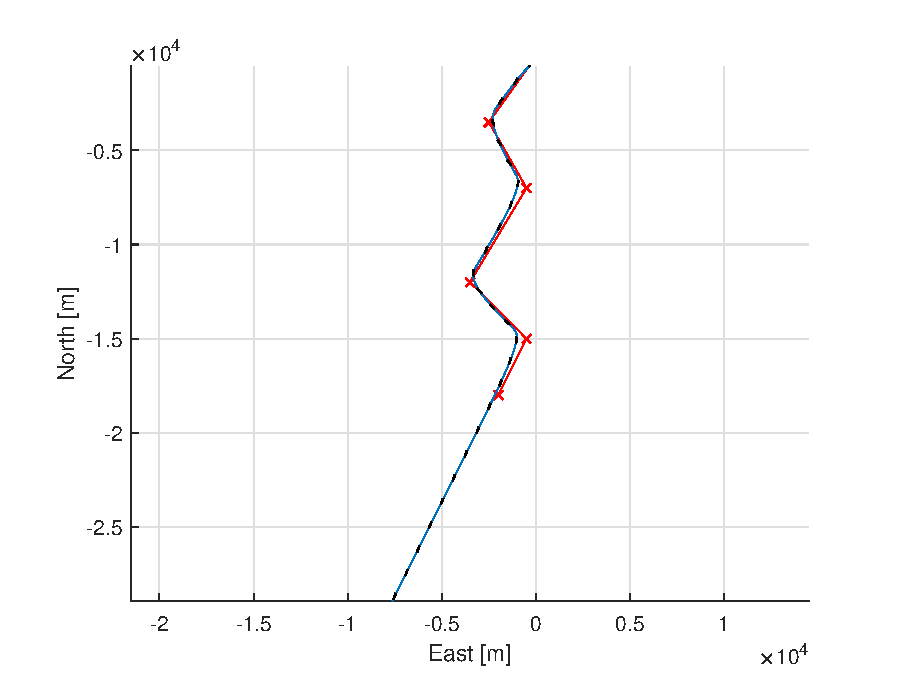
\includegraphics[width=\textwidth]{path_2_2}
		\caption{Path and waypoints}
		\label{fig:path_2_2}
	\end{subfigure}%
        ~
	\begin{subfigure}[b]{0.4\textwidth}
		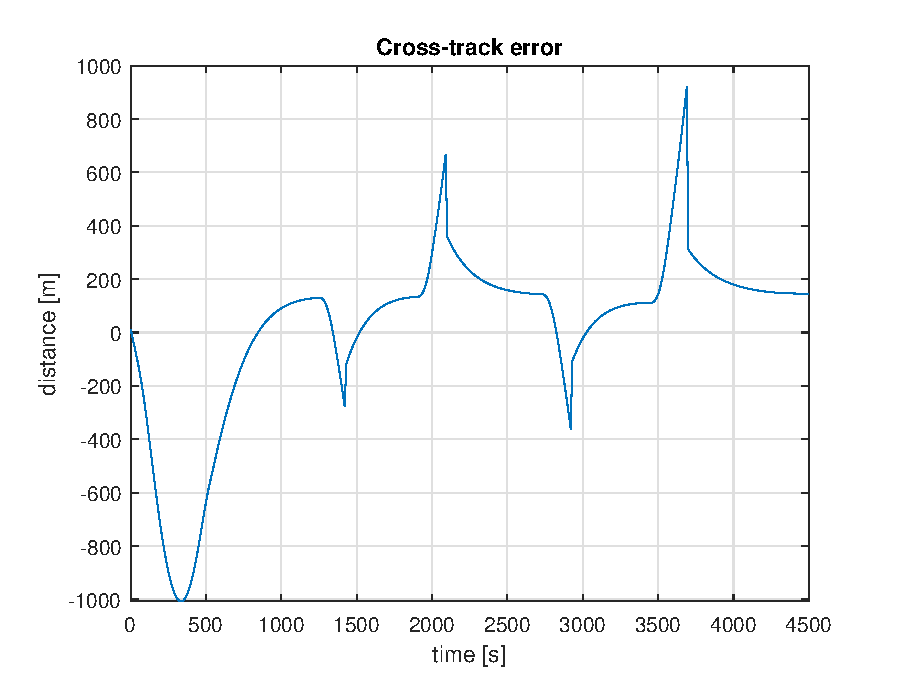
\includegraphics[width=\textwidth]{cross_track_error2_2}
		\caption{Rudder with saturation}
		\label{fig:cross_track_error2_2}
	\end{subfigure}
	\caption{Cross-track error}
	\label{fig:task2_2}
\end{figure}

\subsection*{Problem 2.3}
The path-following is not really working as expected, as the 
